%%
%% (
%%  )\ )                             (
%%  (()/(   (            (             )\  )   (
%%   /(_))  ))\   (       ))\  (   (   (()/(   ))\
%%   (_))  /((_)  )\  )  /((_) )\  )\   ((_))/((_)
%%   | _ \(_))(  _(_/( (_) )  ((_)((_)  _| |(_))
%%   |   /| || || ' \))/ -_)/ _|/ _ \/ _` |/ -_)
%%   |_|_\ \_,_||_||_| \___|\__|\___/\__,_|\___|
%%

\documentclass{article}
\usepackage[utf8x]{inputenc}
\usepackage{amsmath}
%\usepackage{slashbox}
\usepackage{amsfonts}
\usepackage{amssymb}
\usepackage{graphicx} % Paquete para incluir imágenes en el documento LaTeX
\usepackage{hyperref}
\hypersetup{
  colorlinks=true,
  linkcolor=blue,
  filecolor=magenta,
  urlcolor=cyan,
}
\urlstyle{same}
\usepackage{varwidth}

\newcommand\tab[1][1cm]{\hspace*{#1}}

\usepackage{multirow}

\usepackage[a4paper,rmargin=1.5cm,lmargin=1.5cm,top=1.5cm,bottom=1.5cm]{geometry}

\usepackage{pdfpages}

\usepackage{xcolor}
\usepackage{minted}
\setminted[cpp]{frame=lines, framesep=2mm, baselinestretch=1.2, rulecolor=\color{black!80},
                bgcolor=DarkGray,fontsize=\normalsize}
\usemintedstyle[cpp]{monokai}
\setminted[python]{frame=lines, framesep=2mm, baselinestretch=1.2, rulecolor=\color{black!80}, bgcolor=DarkGray}
\usemintedstyle[python]{monokai}
\setminted[java]{frame=lines, framesep=2mm, baselinestretch=1.2, rulecolor=\color{black!80}, bgcolor=DarkGray}
\usemintedstyle[java]{monokai}
\setminted[javascript]{frame=lines, framesep=2mm, baselinestretch=1.2, rulecolor=\color{black!80}, bgcolor=DarkGray}
\usemintedstyle[javascript]{monokai}
\setminted[php]{frame=lines, framesep=2mm, baselinestretch=1.2, rulecolor=\color{black!30}, bgcolor=LightGray}
\setminted[html]{frame=lines, framesep=2mm, baselinestretch=1.2, rulecolor=\color{black!30}, bgcolor=LightGray}
\setminted[bash]{baselinestretch=1.2,rulecolor=\color{black!30},fontsize=\footnotesize,bgcolor=LightGray}
\definecolor{LightGray}{gray}{0.98}
\definecolor{DarkGray}{gray}{0.1}
\definecolor{MidGray}{gray}{0.8}
\definecolor{codegreen}{rgb}{0,0.6,0}
\definecolor{codegray}{rgb}{0.5,0.5,0.5}
\definecolor{codepurple}{rgb}{0.58,0,0.82}
\definecolor{backcolour}{rgb}{0.95,0.95,0.92}

%% \setlength{\parindent}{0px}  % Setea la indentacion de la primera linea de cada parrafo a cero pixeles.


\title{Introducción a JavaSE}
\author{@RuneCode}

\begin{document}
%% Portada
\includepdf{./portada/portada.pdf}

%% Clase 1
\section{Eliminando kernels antiguos en Fedora}%
Cuando se actualiza el sistema con Fedora a veces ocurre el siguiente error:

\begin{figure}[h!]
  \centering
  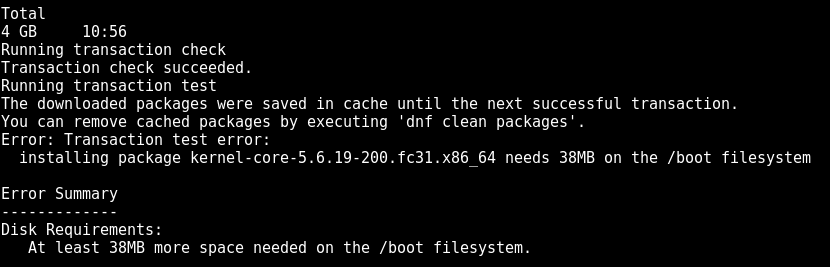
\includegraphics[scale=0.75]{./Pictures/001_error.png}
\end{figure}

Esto sucede porque la partición boot se encuentra llena, entonces lo que
tenemos que hacer es eliminar los kernels antiguos para liberar espacio.\\

Primero vamos a revisar con qué kernel iniciamos nuestro sistema:

\begin{minted}{bash}
  uname -r
\end{minted}

\begin{figure}[h!]
  \centering
  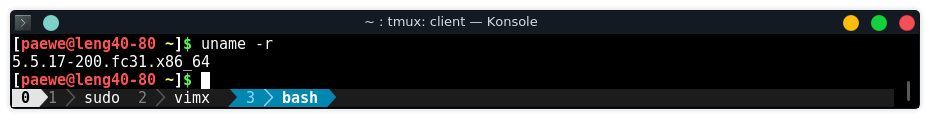
\includegraphics[scale=0.75]{./Pictures/002_uname.png}
\end{figure}

Para listar los paquetes que tenemos instalados usamos:

\begin{minted}{bash}
  rpm -qa
\end{minted}

Si queremos filtrar los que tienen \textbf{kernel} en su nombre, usamos un pipe
con grep y la palabra kernel.

\begin{minted}{bash}
  rpm -qa | grep -i kernel
\end{minted}

\begin{figure}[h!]
  \centering
  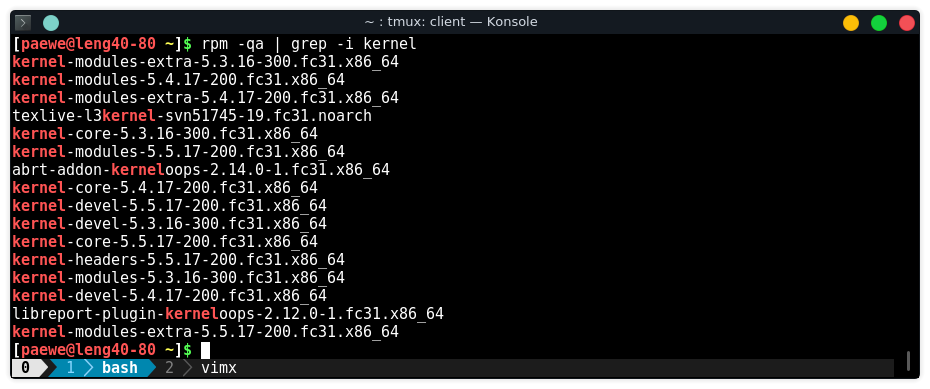
\includegraphics[scale=0.75]{./Pictures/002_rpm_kernel.png}
\end{figure}

Para este caso vemos tres versiones del kernel, de las que eliminaremos dos
versiones dejando solo la que estamos usando.\\

\newpage

Para eliminar una de las imagenes usamos lo siguiente:

\begin{minted}{bash}
  sudo dnf remove kernel-*5.4.17-200*
\end{minted}

\begin{figure}[h!]
  \centering
  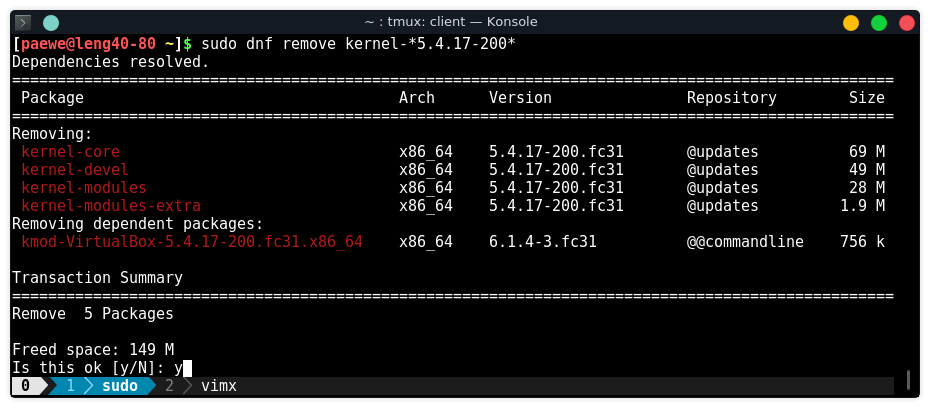
\includegraphics[scale=0.75]{./Pictures/003_dnf_remove_kernel.png}
\end{figure}

Luego de eliminar las imágenes podemos filtrar nuevamenten los paquetes kernel
que tenemos instalados.

\begin{figure}[h!]
  \centering
  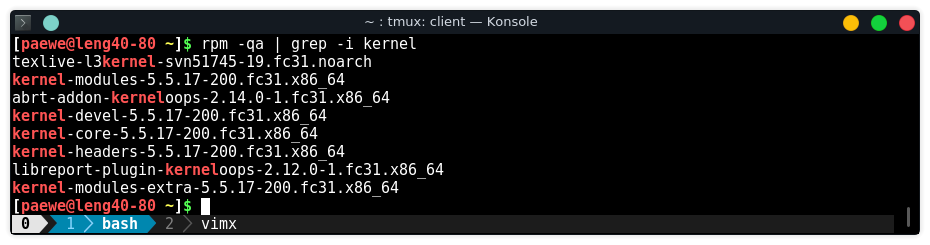
\includegraphics[scale=0.75]{./Pictures/004_only_one_image.png}
\end{figure}

Luego podemos proseguir con la actualización del sistema.

\begin{figure}[h!]
  \centering
  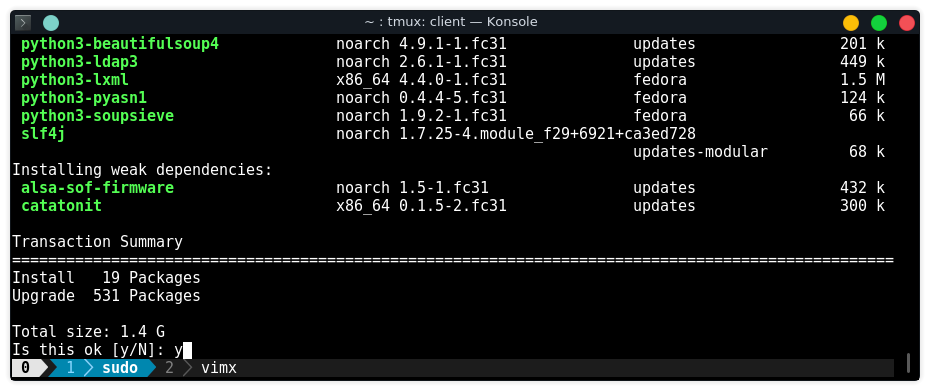
\includegraphics[scale=0.75]{./Pictures/005_update_ok.png}
\end{figure}

\begin{figure}[h!]
  \centering
  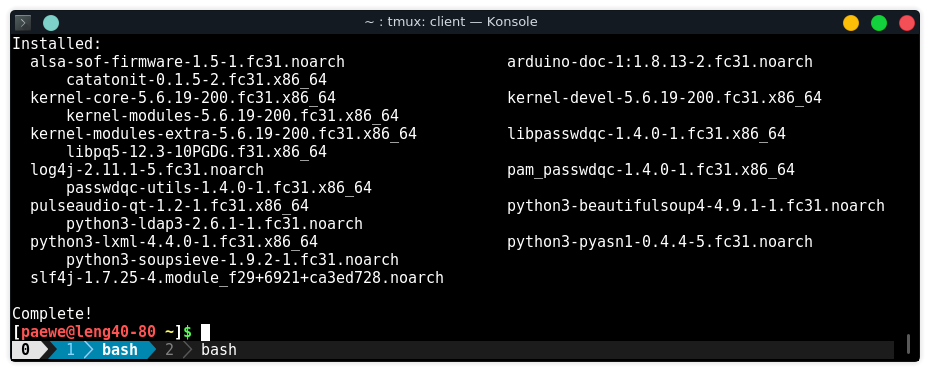
\includegraphics[scale=0.75]{./Pictures/006_update_ok.png}
\end{figure}


\end{document}

